%!TEX root = ../documentation.tex

\chapter{Benutzeroberfläche}

\section{Beschreibung der Benutzeroberfläche}
\subsection{Appstart}
Nach dem erstmaligen Start der App durch anklicken des App Icons gelangt der Benutzer zur in Abbildung \ref{label:startview} gezeigten Benutzeroberfläche.

\begin{figure}[H]
\centering
	\begin{minipage}{0.4\textwidth} 
	\centering
	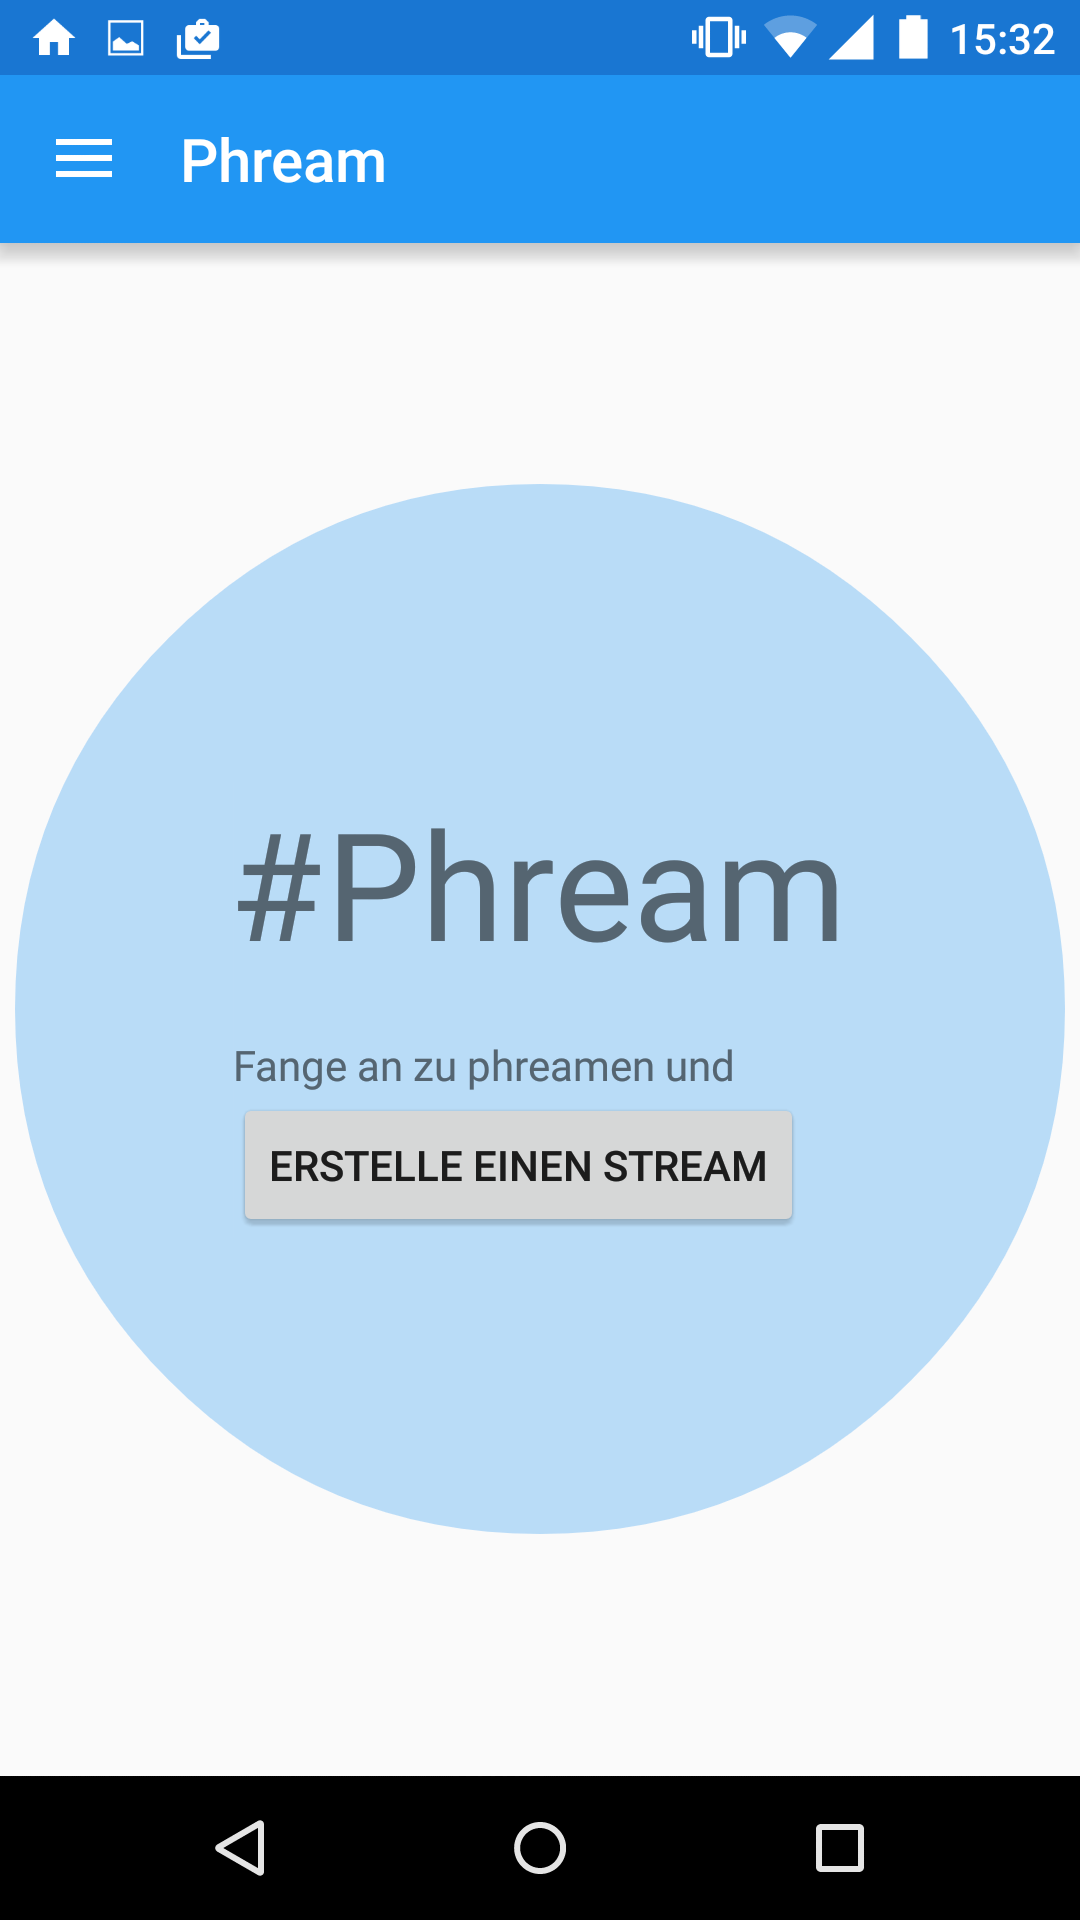
\includegraphics[width=0.6\textwidth]{images/screenshots/startview.png}
	\caption{App-Startansicht}
	\label{label:startview}
	\end{minipage}
	\hfill
	\begin{minipage}{0.4\textwidth}
	\centering
	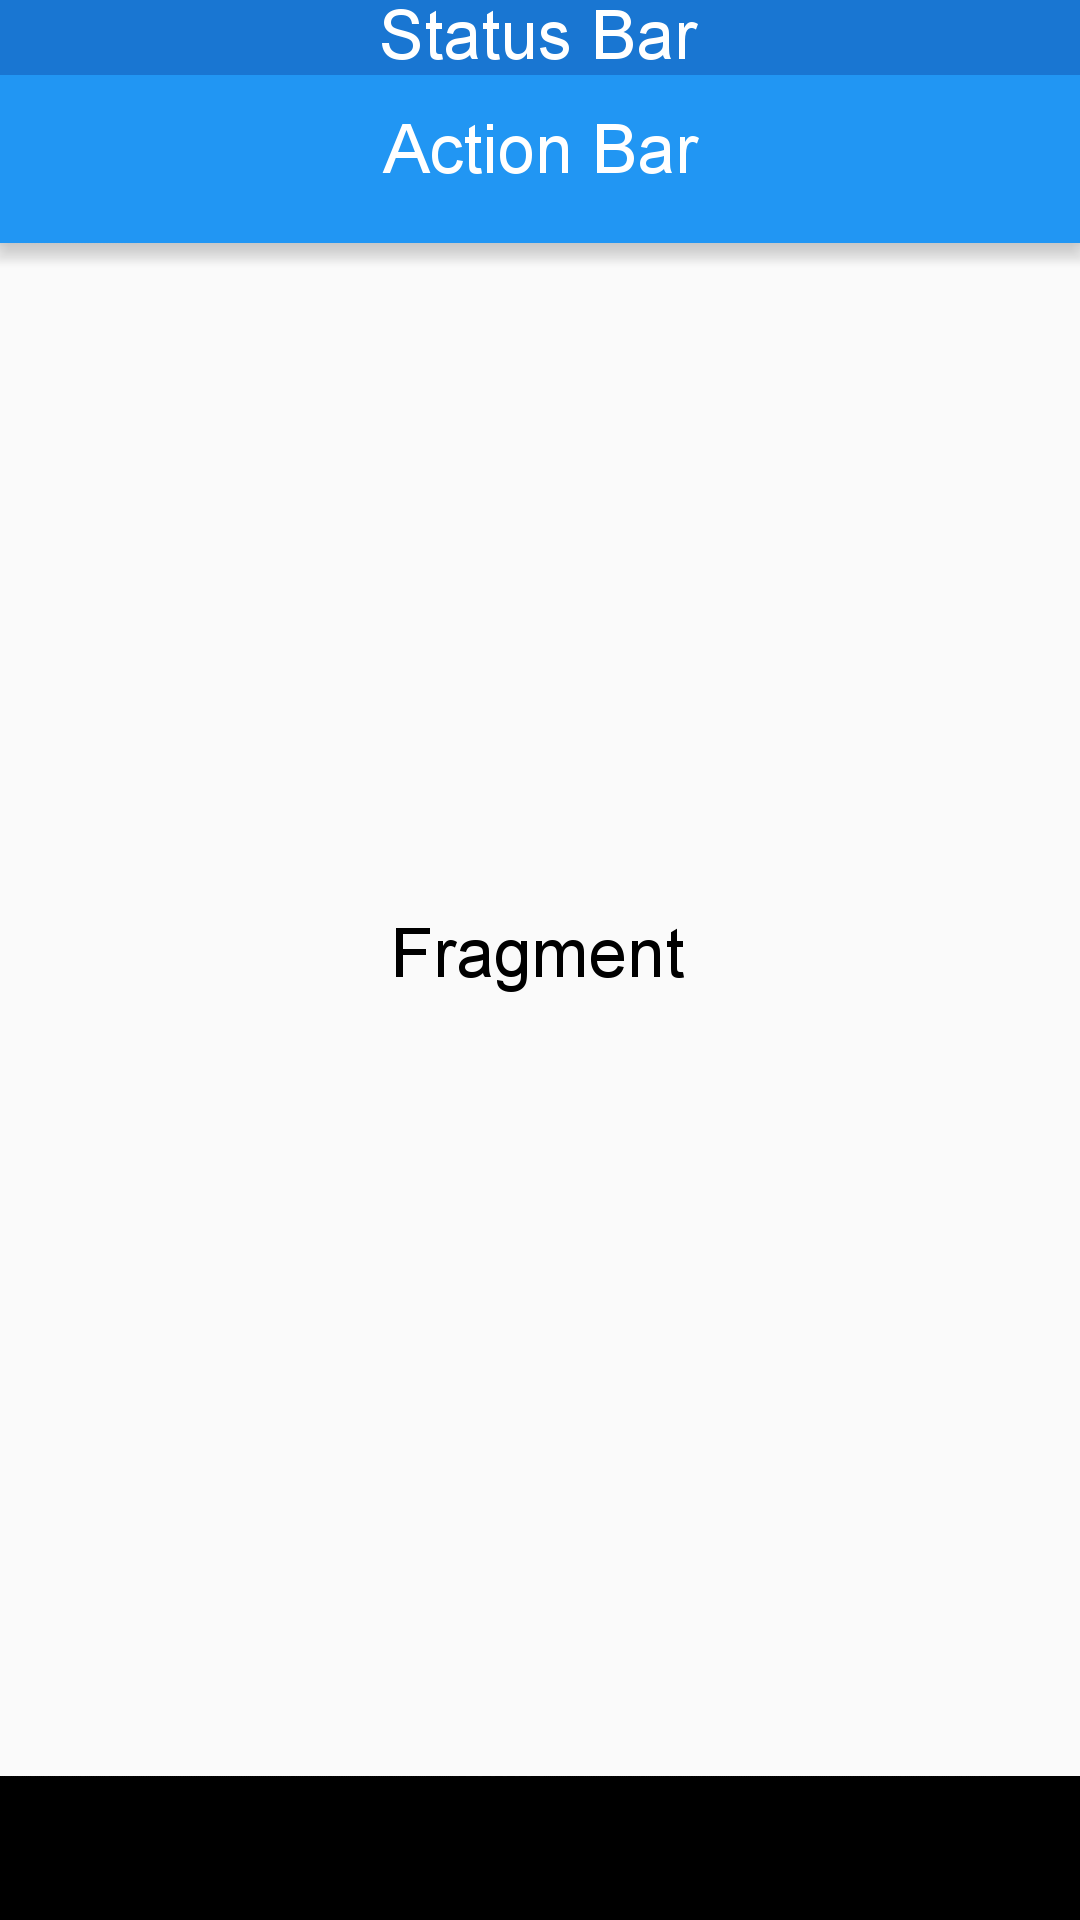
\includegraphics[width=0.6\textwidth]{images/screenshots/startview_schema.png}
	\caption{Schematische Darstellung}
	\label{label:startview_schema}
	\end{minipage}
\end{figure}
Die in Abbildung \ref{label:startview_schema} eingezeichnete Statusbar ist standardmäßig in jeder Ansicht der App zusehen und zeit allgemeine Statusinformationen zum Androidgerät an. Die Action Bar wird von der App selbst gestaltet und beinhaltet verschiedene Optionen, wie beispielsweise Menüs. Die größten Teil der App nimmt das Fragment in Anspruch. In diesem werden die verschiedenen Informationen der App dargestellt. Das Fragment ist dabei eine Art selbständige \enquote{Sub-Activity}, die einen eigenen Lifecycle, inklusive eigener Action Listener.
Das Fragment wird dynamisch durch einen Manager bei Benutzeraktionen ausgetauscht.

In der aktuell angezeigten Startansicht (Abbildung \ref{label:startview}), die beim erstmaligen Start oder wenn Stream (Ordner) angelegt angezeigt wird, beinhaltet das Fragment den dargestellten Text, den Button zum anlegen eines Streams und den im Hintergrund platzierten Kreis. Durch anklicken des Buttons, öffnet sich ein Eingabefenster, in dem ein neuer Streamname eingegeben werden kann. Nach Bestätigung des Streamnamens wird der Stream angelegt und erscheint daraufhin in Navigation Drawer. 

\subsection{Navigation Drawer}

Der Navigation Drawer (Abbildung \ref{label:navigationdrawer}) kann durch klicken auf das Menüicon oben links neben dem Appnamen oder durch einen Swipe vom linken Bildschirmrand geöffnet werden.
In der daraufhin eingeblendeten Ansicht hat der Benutzer die Möglichkeit zwischen verschiedenen Streams zu wechseln und neue Streams anzulegen. Durch anklicken eines Streamnamens wird dieser aktiv und wird daraufhin in der Hauptansicht angezeigt. Durch einen swipe zum linken Bildschirmrand oder durch anklicken des Pfeils links neben dem Appnamen kann der Navigation Drawer geschlossen werden.

\begin{figure}[H]
\centering
	\begin{minipage}{0.4\textwidth} 
	\centering
	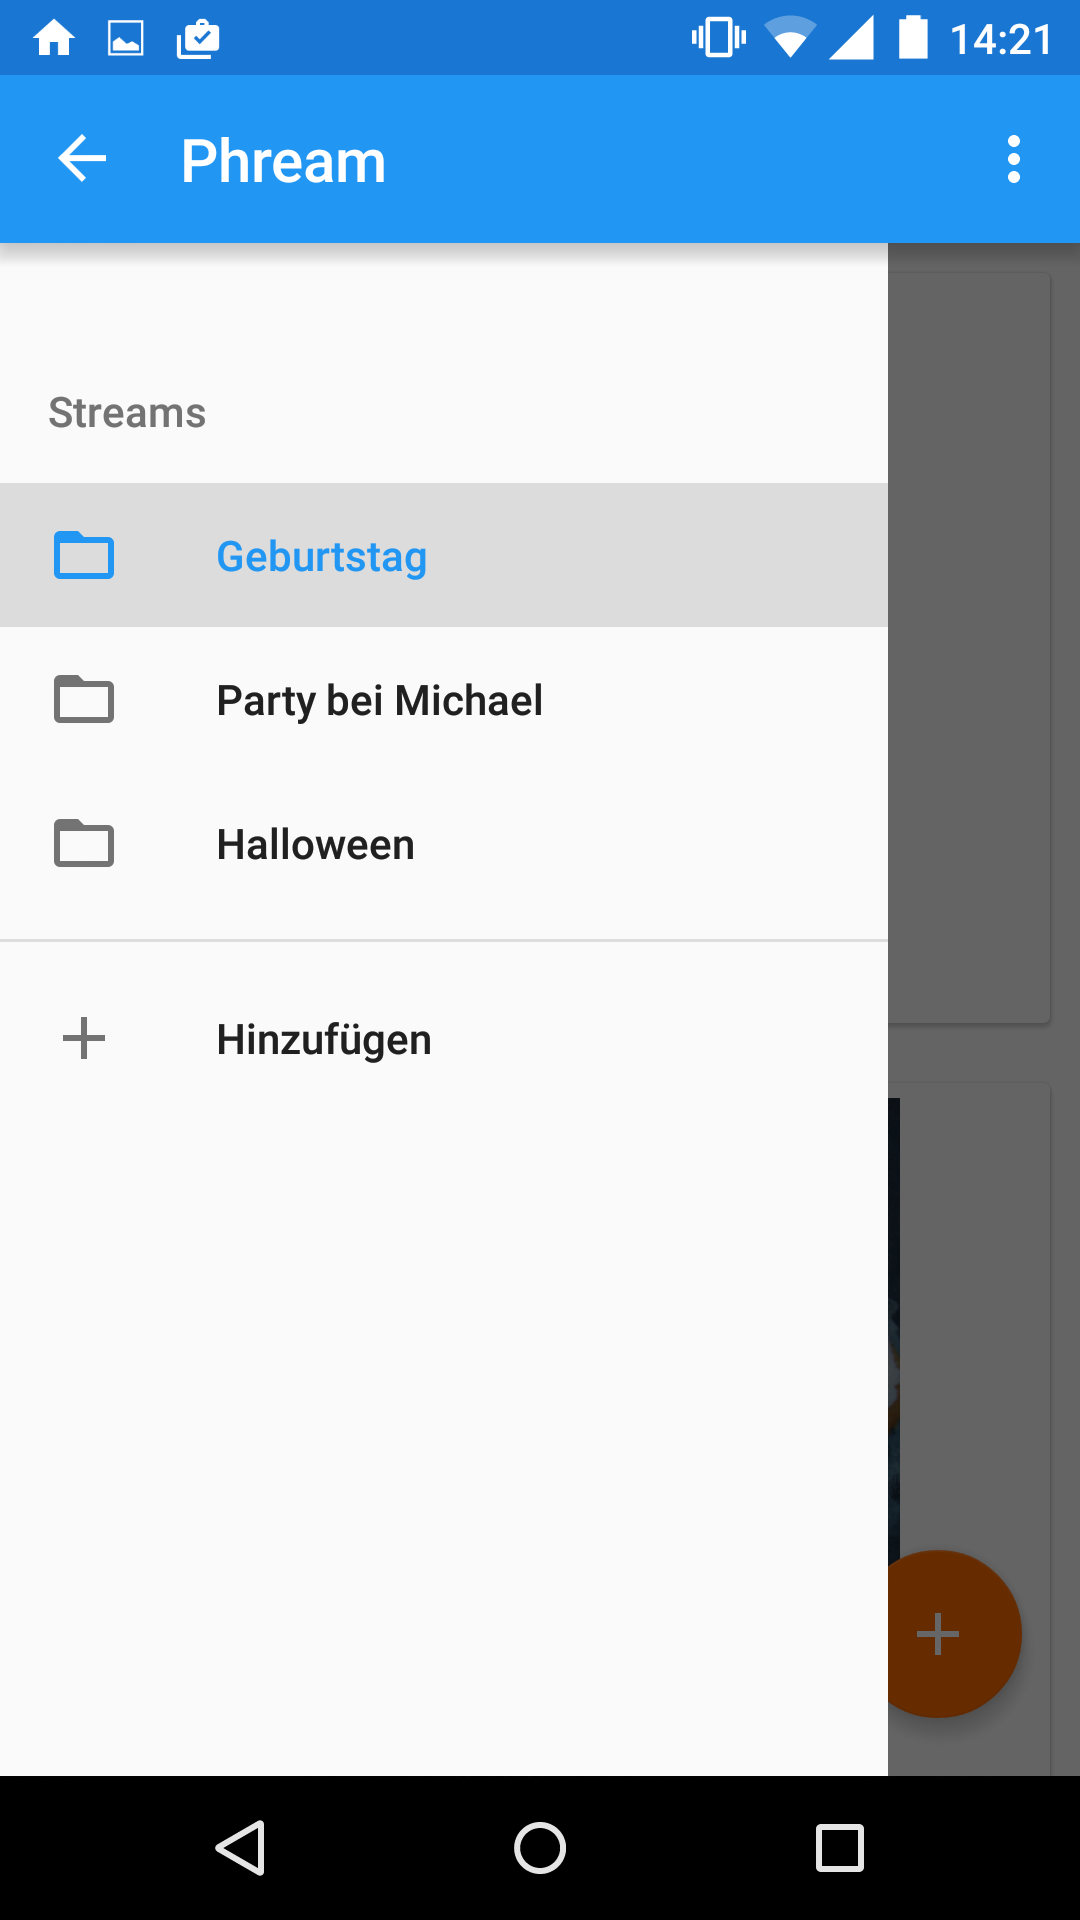
\includegraphics[width=0.6\textwidth]{images/screenshots/navigationdrawer.png}
	\caption{Navigation Drawer}
	\label{label:navigationdrawer}
	\end{minipage}
	\hfill
	\begin{minipage}{0.4\textwidth}
	\centering
	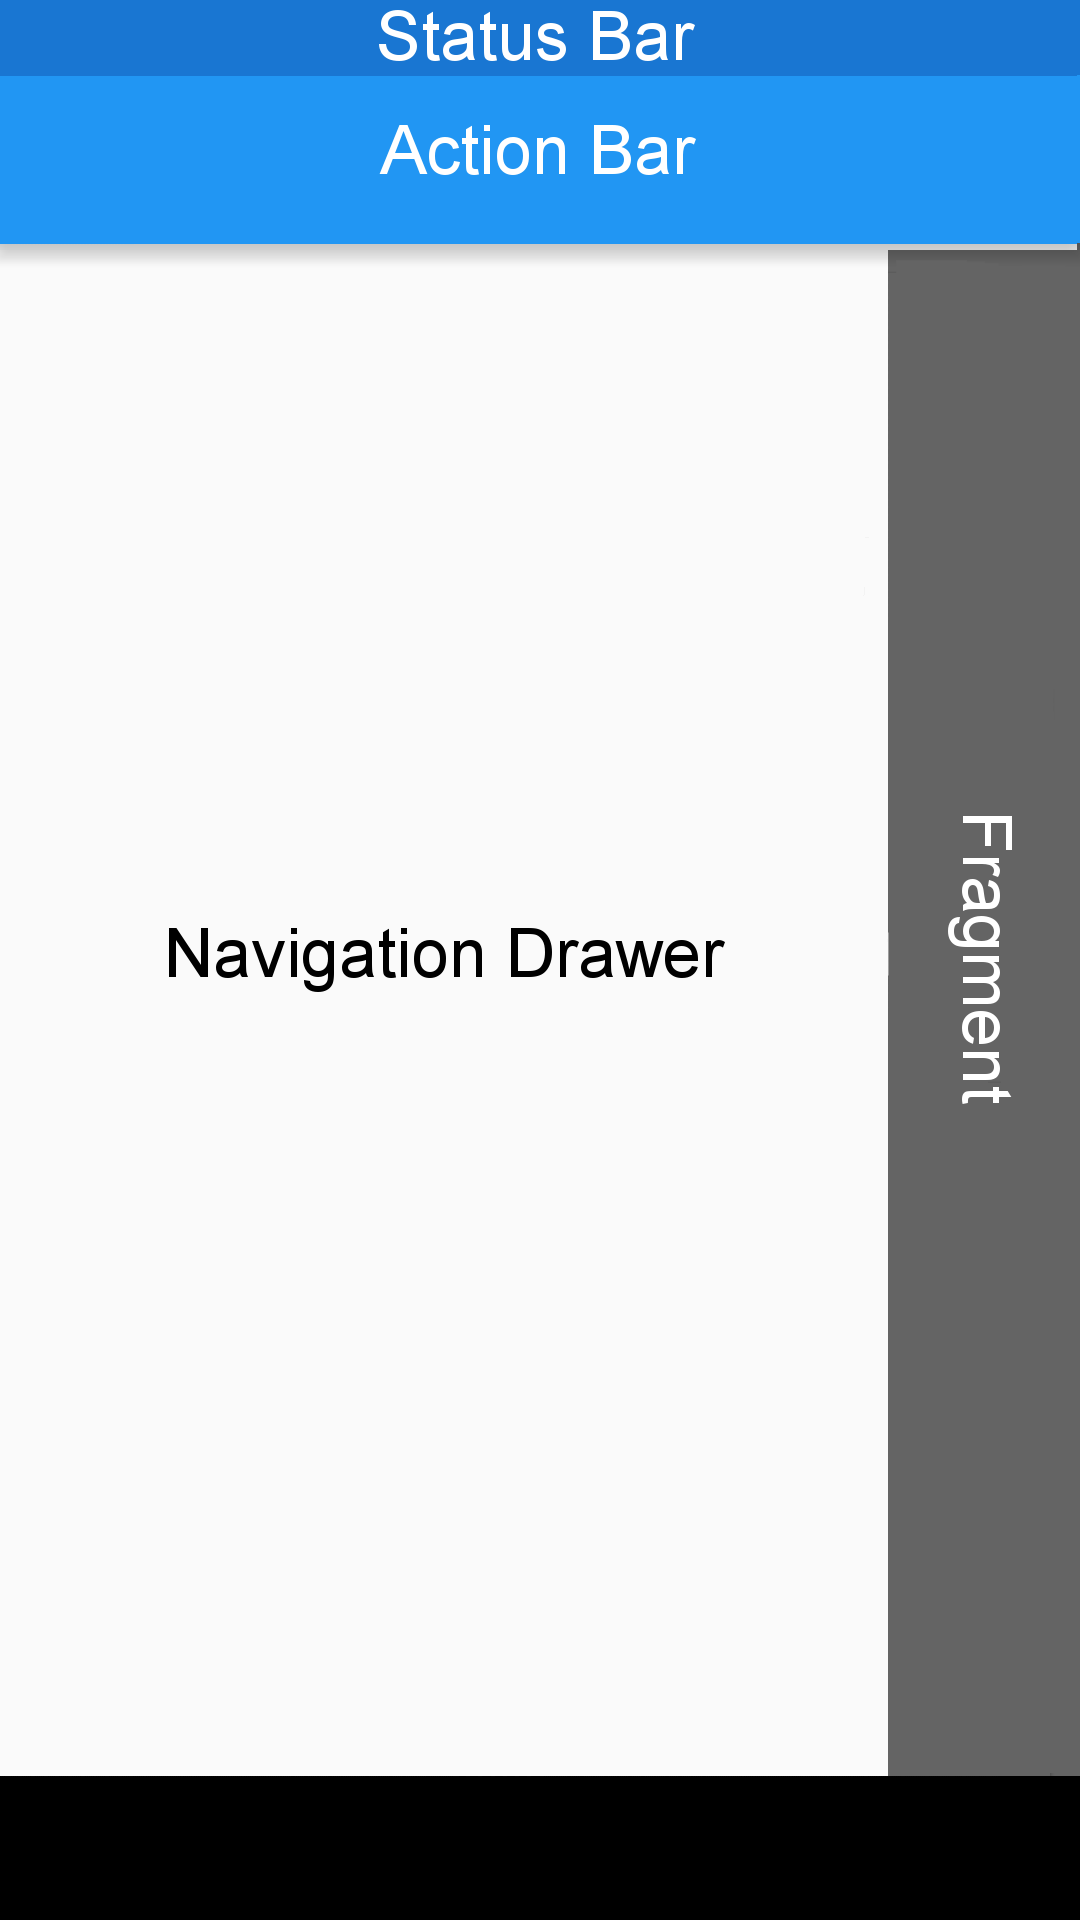
\includegraphics[width=0.6\textwidth]{images/screenshots/navigationdrawer_schema.png}
	\caption{Schematische Darstellung}
	\label{label:navigationdrawer_schema}
	\end{minipage}
\end{figure}
In der schematischen Darstellung (Abbildung \ref{label:navigationdrawer_schema}) ist zu sehen, dass der Navigation Drawer das aktuelle Fragment \enquote{überdeckt} und den restlichen Teil des Fragments abdunkelt. In der Action Bar wird dabei der Button zum öffnen des Navigation Drawer zu einem Pfeil.

\section{Verwendete Libraries}